%!TEX program = xelatex
\documentclass[9pt, compress]{beamer}
\usetheme[titleprogressbar]{m}

\usepackage{booktabs}  
\usepackage[scale=2]{ccicons}
\usepackage{minted}
\usepgfplotslibrary{dateplot}
\usemintedstyle{trac}
\author{\textbf{Дырночкин Александр}} 
\title{Разработка подходов и методов обработки и извлечения библиографической информации из научной электронной библиотеки elibrary}

\institute{\textbf{Ульяновский государственный технический университет}}
\date{}

\begin{document}
	\maketitle
	
	\begin{frame}
		\frametitle{Цель исследования}
		\begin{quotation}
			Целью работы является разработка подходов и методов обработки и извлечения библиографической информации,  для последующего наукометрического анализа публикаций и формирования научных групп по заданной тематике, на основе данных об авторах.
		\end{quotation}
	\end{frame}
	
	\begin{frame}
		\frametitle{Объект и предмет исследования}
		\begin{quotation}
			Объектом исследования является информация по публикациям различных авторов из цифровых библиографических и реферативных базы данных. Такие базы представляют собой инструмент для отслеживания цитируемости статей, опубликованных в научных изданиях. Также они являются одним из главных источников получения наукометрических данных для проведения оценочных исследований.
		\end{quotation}
		
		\begin{quotation}
			Предметом исследования является библиографическая информация по сотрудникам УлГТУ из научной электронной библиотеки elibrary.
		\end{quotation}
	\end{frame}

	\begin{frame}
		\frametitle{Задачи}
		Достижение поставленной цели предполагает реализацию следующих задач:
		\begin{itemize}
		    \item анализ и исследование существующих моделей, алгоритмов и методов интеллектуального анализа и кластеризации текстов
			\item проектирование аглоритма извлечения и структуризации библиографических данных с сайта elibrary.ru
			\item формализация и прототипирование алгоритма интеллектуального анализа текста, для формирования научных групп
			\item проведение экспериментов с полученным прототипом системы
		\end{itemize}
	\end{frame}	
	
	\begin{frame}
		\frametitle{Научная новизна}
		\begin{quotation}
			Научная новизна работы состоит в гибридизации алгоритмов интеллектуального анализа текстов и кластерного анализа для формирования научных (ученых) групп  на основе библиографической информации.
		\end{quotation}
	\end{frame}

	\begin{frame} 
	    \begin{quotation}
			Исходными данными системы являются научные идентификаторы сотрудников УлГТУ. На основании которых будет загружена информация по всем сатьям автора из elibrary.
		\end{quotation}
		\frametitle{Исходные данные системы}
		\begin{figure}
        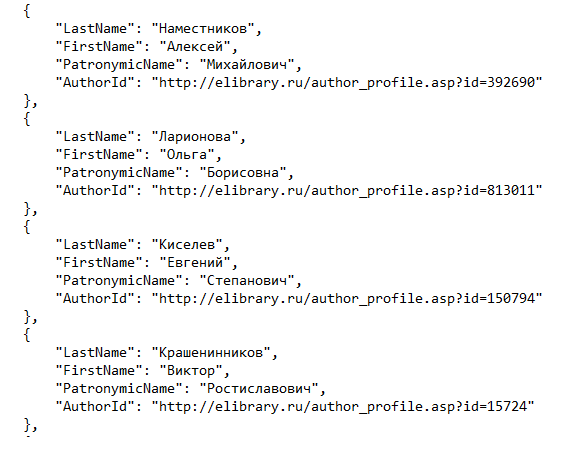
\includegraphics[width=190pt,height=150pt]{img/inputdata.png}
        \caption{Исходные данные}
		\end{figure}
	\end{frame}
	
	\begin{frame} 
		\frametitle{Описание схемы формарования начных групп}
		\begin{figure}
        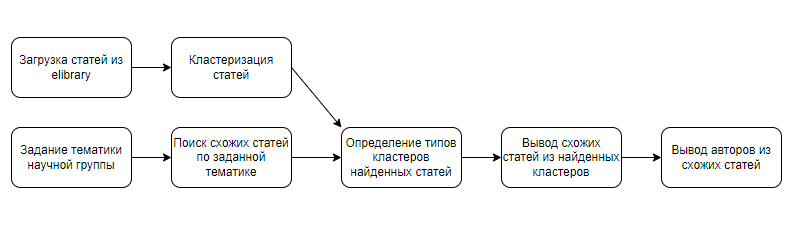
\includegraphics[width=\textwidth,height=125pt]{img/alg.png}
        \caption{Схема формирования научных групп}
		\end{figure}
	\end{frame}
	
	\begin{frame} 
		\frametitle{Положение выносимые на защиту}
		\begin{itemize}
		    \item алгоритм извлечения информации по авторам с сайта elibrary
			\item алгоритм интеллектуального анализа текстов и кластерного анализа для формирования научных (ученых) групп  на основе библиографической информации.
			\item механизм формирования графа соавторов
		\end{itemize}
	\end{frame}
	
	\begin{frame} 
		\frametitle{Обзор научных работ по схожей тематике}
		\begin{itemize}
		    \item Кластеризация текстовых документов из электронной базы публикаций алгоритмом FRiS-Tax. Н.Г. Загоруйко, В.Б. Барахнин, И.А. Борисова, Д.А. Ткачёв
			\item Тематическая кластеризации научной литературы. А.В. Николаев, В.В. Жуков
			\item Обзор и экспериментальное сравнение методов кластеризации текстов. П.А. Пархоменко, А.А. Григорьев, Н.А. Астраханцев
		\end{itemize}
	\end{frame}
\end{document}